Based on a paper: Autonomously Generating Hints by Inferring Problem
Solving Policies \cite{piech2015autonomously} \\ \emph{Learning at Scale 2015.}

\vspace{7mm}

\begin{figure}[h!]
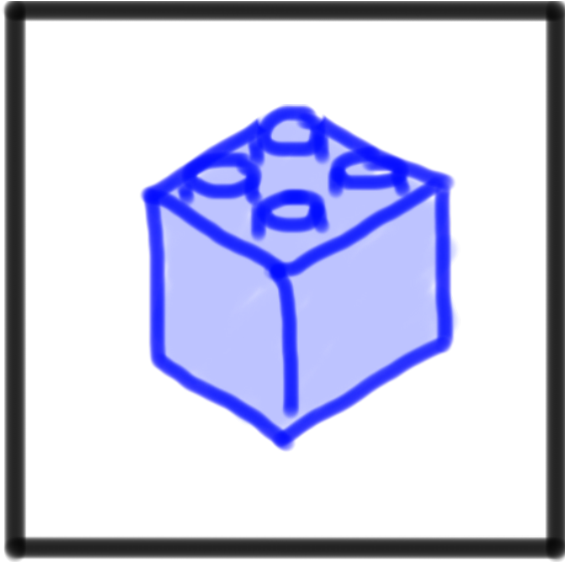
\includegraphics[width=0.2\textwidth]{img/assnType_2}
\end{figure}

\vspace{7mm}

When students solve challenges that involve layered steps of problem solving -- for example when they solve programming assignments -- the trajectory that they take to navigate to their final answer contains rich information about what they know. In fact, in order to understand students we believe it would be more fruitful to observe \emph{how} they solve a problem  then just to look at their final answer. In order to take this next, deeper step into understanding how student learn we chose to study students working on Maze Programming Assignments. These assignments which are designed for K-12 students and use blocks that represent standard control flow paradigms (like repeat, while and if) are ideal because the number of unique programs that students generate is quite small, and thus easier to understand.

%Deep Knowledge tracing is a powerful tool for the domain of assignments where student responses can be encoded as ``correct" or ``incorrect". For more complex domains where students produce rich, structured responses it is no longer sufficient to simply track their work on the granularity of one binary input per assignment. When a student solves a richly structured assignment they produce a series of partial solutions and need assistment intermediately.
%In this domain we focus on predicting what a teacher would do.
%One of the reasons that I believe recurrent neural networks are hard to apply to the task of tracing knowledge as a student works on a multi stage assignment is that predicting what a student will do next is particularly difficult given the sparsity of the solution space.

Exploring the whole sequence of steps a student takes to produce work, and the patterns that emerge from thousands of such sequences is fertile ground for a richer understanding of learning. In this chapter uncover a pattern in student learning that can both predict the way an expert teacher would encourage a student to make forward progress and predict a student's future retention. We discovered this pattern by observing historical data of students learning in the Code.org `Hour of Code,' curriculum (which is to the best of our knowledge the largest online course to date). The approached this problem by first focussing on trying to find patterns that allow us to predict how teachers would suggest students make forward progress. Such a prediction can form the basis for an effective hint generation system. The algorithms that we develop are more accurate than current state-of-the-art methods at recreating expert suggestions, are easy to implement and scale well. We then show that the same framework which motivated the hint generating algorithms suggests a sequence-based statistic that can be measured for each learner. We discover that this statistic is highly predictive of a student's future success. 

A motivating case study is the set of assessments in the Code.org Hour of Code course. Code.org is a non-profit organization that led a coordinated effort to have every K-12 student in the United States complete an hour worth of computer science. As part of the initiative Code.org hosted an Hour of Code curriculum: a series of twenty introductory programming ``challenges" with instructional videos. In the year and a half since they launched, over 27 million learners have tried their curriculum and it has been taught in over 90 thousand classrooms making it, to the best of our knowledge, the largest MOOC to date. In the challenges students generate programs by putting together blocks of code. The open ended nature of coding, and the many avenues that students can take to get to the solution both make the challenges appealing learning activities, and prevent Code.org from being able to provide expert feedback to stuck students. 

The Hour of Code challenges take several steps for a student to solve. At each point in time, the student's current work constitutes a partial solution $\psi \in S$ where $S$ is the set of all possible responses. As the student works on the assessment they will transition through a series $T = \{\psi_0, \psi_1, ... , \psi_n$\} of partial solutions from step $0$, when they have done no work, to step $n$ when they have either reached the solution or given up. 
We propose that generating feedback autonomously for an assessment of this nature can be seen as the composition of two tasks: 
\begin{enumerate}
\item Deciding for any learner what partial solution an educational expert would suggest they transition to next. 
\item Choosing how to communicate that information to the student such that they improve on a learning objective. 
\end{enumerate}
We suggest that both of the decoupled tasks can be solved and tested independently. The objective of this paper is to solve the former problem by learning what we call a Problem Solving Policy (PSP): a decision for any partial solution as to what next partial solution a student should take (see definition \ref{pspDef} and the example in figure \ref{fig:policy}). Using historical data we generate PSPs for challenges in the Hour of Code and evaluate to what extent they capture expert opinion.

\begin{defo}
Problem Solving Policy (PSP). \\ 
Let $S$ be the set of partial solutions.
A problem solving policy $\pi : S \rightarrow S$ specifies a partial-solution $s' = \pi(s)$ for all $s \in S$.
\label{pspDef}
\end{defo}

\begin{figure}
\centering
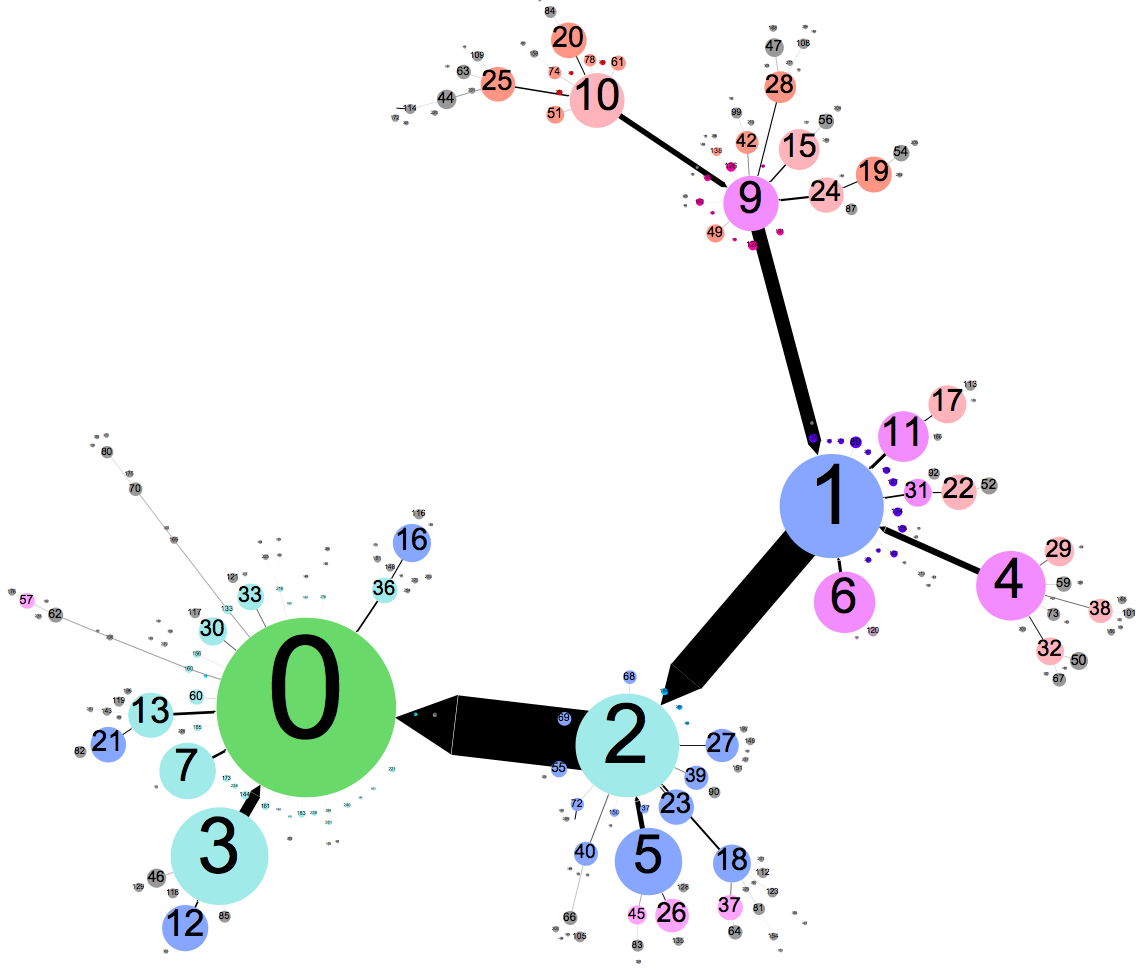
\includegraphics[width=1.0\columnwidth]{img/policy3}
\caption[Example problem solving policy]{A visualization of a problem solving policy generated for an early Hour of Code challenge. Each node is a unique partial solution, node 0 is the correct answer. The edges show what next partial solution we think an expert would suggest students move towards.}
\label{fig:policy}
\end{figure}


Note that the definition for a PSP makes the Markov assumption as no partial solution other than a student's current state is considered in the policy mapping. 

A PSP provides a foundation for generating formative feedback. For a given partial solution, there are many types of issues a student could have: they may have missed a step, made a mistake, have compounded mistakes, or possibly they are on the right path and simply need to keep going. An ideal PSP captures these diverse needs. It selects the single part of the partial solution the student should work on first and denotes how they should do so. Importantly, the PSP can also be evaluated independently from the actual feedback given to students (e.g. via a hint generation) given a ground truth dataset composed of expert evaluations on how they would push a student forward. 

Our hypothesis is that for large classes like Code.org there are patterns which materialize in how the many previous students have navigated from an empty project to the final answer which can be leveraged to learn how students should move forward from any $\psi \in S$. For example, if ten thousand students had at some point all submitted the exact same partial solution with the same set of mistakes, it seems reasonable that the best way forward is illuminated by the way that crowd then went on to fix their programs. Surprisingly, we found that many of the most obvious statistics that could be calculated from historical data or static analysis were not particularly useful. 


The main contributions of this work are:
(1) a family of algorithms which can accurately predict how experts believe learners should make forward progress from a partial solution (a PSP), based on historical data (2) a related per-student statistic generated from how a student solves a challenge that correlates strongly with future performance and (3) a unified comparison of previously published algorithms. These results speak to a deeper theme: \emph{how} students solve assignments is an under utilized, important lens into what students know and what feedback future students will need.

\section{Related Work}

Giving automated hints for richly-structured assessments at scale is a task with a long history of research that includes fields as diverse as intelligent tutors, theorem provers, crowd sourcing and peer grading.

This work expands upon research towards data-driven PSPs by the Intelligent Tutor (IT) community. In particular a similar problem was posed in Rivers' and Koedinger's paper Automating Hint Generation with Solution Space Path Construction \cite{rivers2014automating}. Rivers et al presented an algorithm which introduces the heuristic that popular partial solutions tend to correspond to good next steps. The Hint Factory by Barnes et al uses a historically trained Markov Decision Problem (MDP) formulation \cite{barnes2008toward}. While both papers present algorithms, the PSPs they generate were not directly measured for quality and the algorithms have previously not been compared to one another. There has been research from the field of static analysis which present alternative ways to generate PSPs. Singh et al suggest ways to find shortest path edits to a solution for programming problems, work which builds off a community of static analysis and theorem prover research \cite{singh2013automated}  \cite{cheang2003automated}. One contribution of this paper is to recreate the IT algorithms and a static analysis algorithm so that we can evaluate them all on the same dataset. 

There are a range of ways to generate feedback for richly-structured assessments at scale that do not involve first learning a PSP. One particularly interesting approach is to crowd source feedback for students \cite{weld2012personalized}, an idea which can be extended to the programming domain \cite{watson2012bluefix}. While it would take a substantial amount of work to give feedback to all answers in rich assessments Nguyen et al suggests ways to identify functionally equivalent programs which can share annotations \cite{nguyen2014codewebs} \cite{rivers2012canonicalizing}. An appealing idea is to have students reflect on what mistakes they made after solving a problem, but this idea does not apply to our setting where students are as young as five years old. At what point is a student ready to consciously reflect on the challenges that they faced? Peer grading is one of the most common solutions for giving feedback to complex assignments at scale in massive open online courses \cite{kulkarni2013peer}; however, it can only be used to give feedback on a final submissions, not hints to a stuck student. Moreover asking students to peer grade programs would have a dramatic impact on the experience of the Hour of Code if used for each challenge.

Cognitive tutors are a compelling approach towards hint generation  \cite{ritter2007cognitive} \cite{aleven2002effective}. They are well rooted in educational theory and have been shown to be pedagogically successful. However, the effort required to author a cognitive model, a necessary component, increases with the number of unique answers a student can produce. For richly-structured assignments such as the one in Code.org this approach does not scale well. Similarly there is a literature of scientists trying to understand, via observation, how student's solve programming challenges. The frameworks developed have engendered better teaching techniques but not at-scale autonomous hints \cite{fitzgerald2008debugging} \cite{ahmadzadeh2005analysis}.

The problem of generating a PSP can be seen as an instance of more general problems. There is a clear parallel between generating a PSP and autonomous decision making \cite{puterman2009markov}. Finding a PSP could be expressed as a route planning task \cite{szczerba2000robust} and historical data could be viewed as item responses where students vote on ways to make forward progress \cite{whitehill2009whose}.  

One of the aims of this work is to enable further comparative research. To this end we will share relevant code and annonomized, aggregate data:
\url{http://stanford.edu/~cpiech/codedotorg.html}

\section{Data}

\begin{figure}
\centering
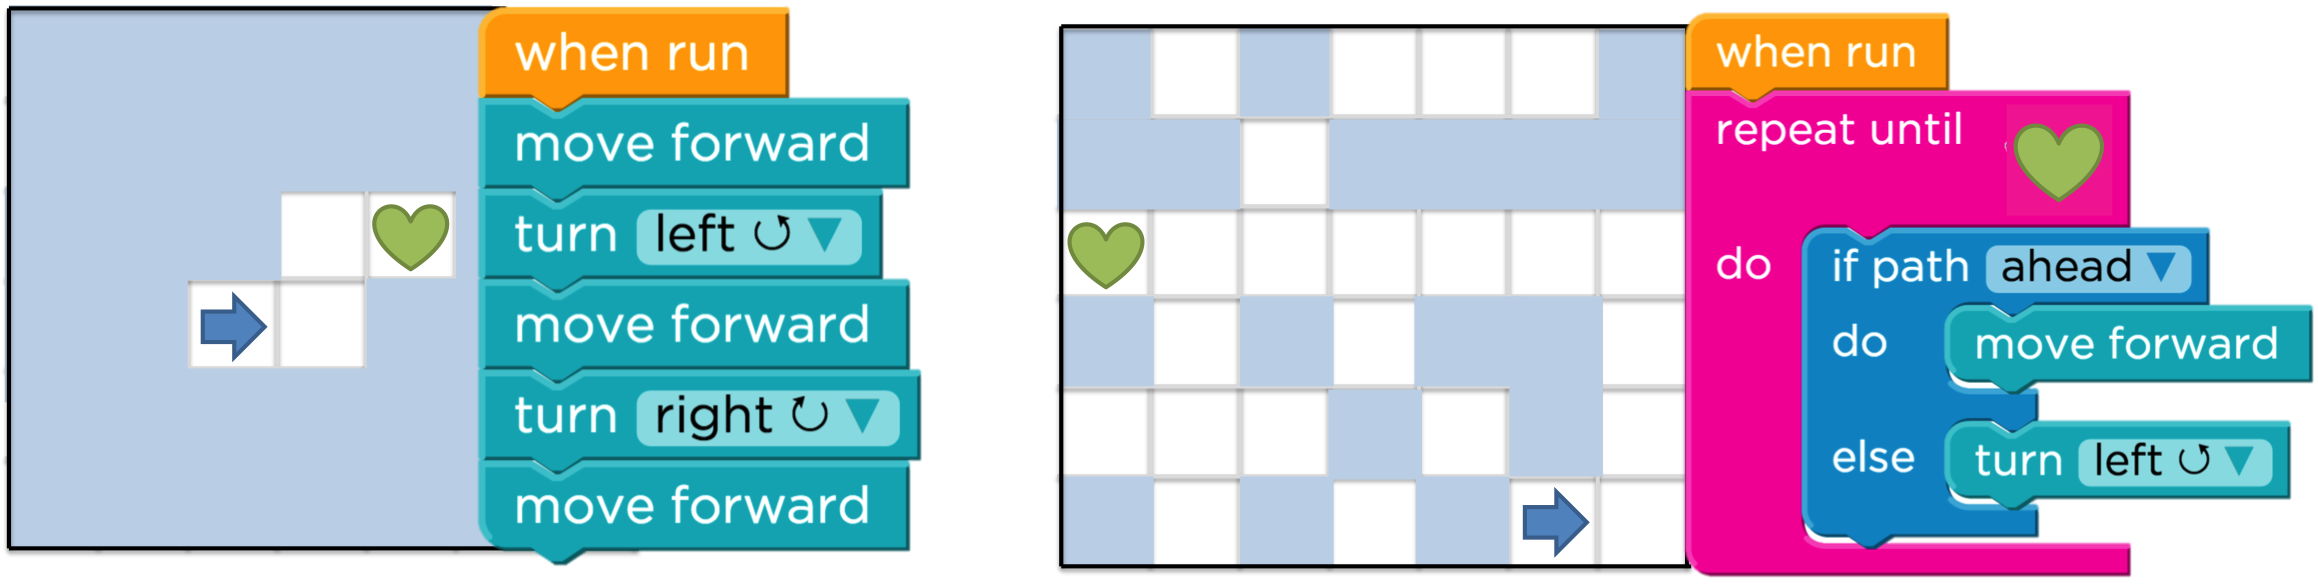
\includegraphics[width=1.0\columnwidth]{img/problems3.png}

\caption[Schematic of Code.org problems]{Schematic of the maze and example solution for \Pa (left) and \Pb (right). The arrow is the agent and the heart is the goal.}
\label{fig:hocExample}
\end{figure}

\begin{figure*}
\centering
\subfigure[]
{
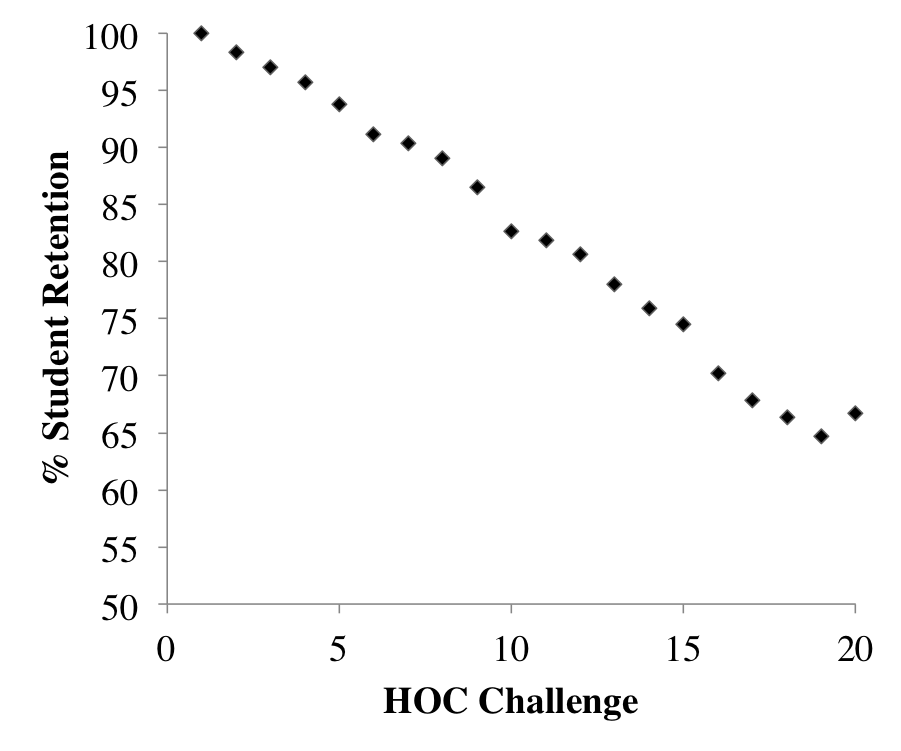
\includegraphics[width=.48\textwidth]{img/retention.png}
\label{fig:retention}
}
\subfigure[]
{
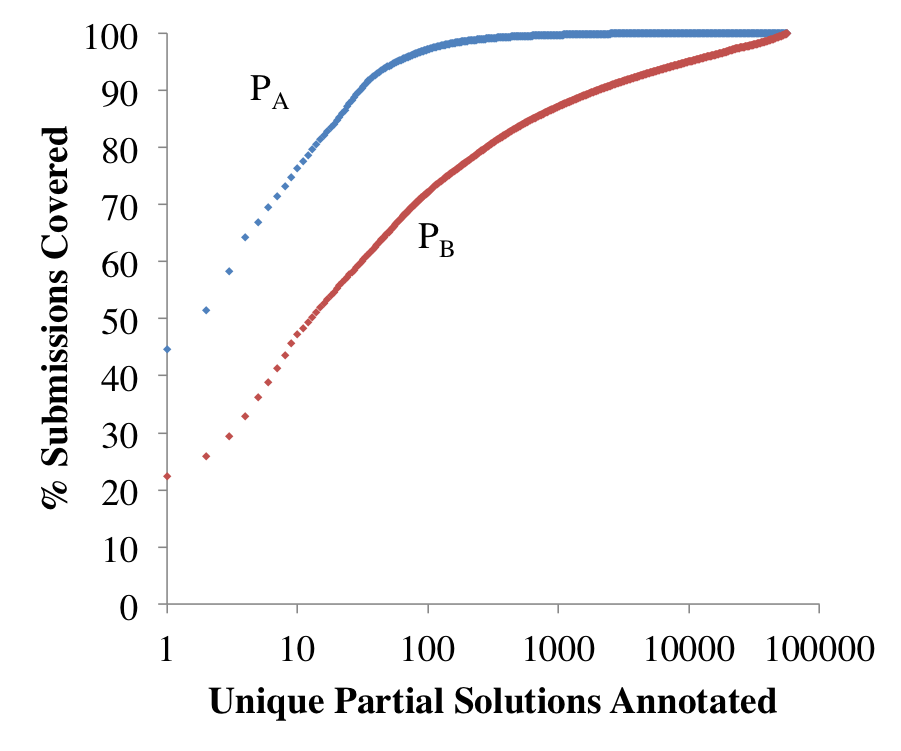
\includegraphics[width=.48\textwidth]{img/annotationImpact.png}
\label{fig:coverage}
}

\caption[Overview of Code.org data]{
\subref{fig:retention} Percent of students who finished the first problem in the hour of code that solve the remaining ones.
 \subref{fig:coverage} The percent of submissions that are covered by annotating the most popular partial solutions. 
 }
\label{tab:predacc}
\end{figure*}


In the Hour of Code website, students write programs to solve maze world puzzles. Each time a learner runs their program, a symbolic representation of their current work is recorded. When the learner submits a final answer, or stops working on a challenge, the learner’s partial solutions are composed into a raw series. There is a simple mechanism to test if two symbolic representations are identical.

The dataset for this paper is the series of partial solutions from all logged in students from December 2013 to March 2014. In that time Code.org gathered over 137 million partial solutions. Retention was quite high relative to other contemporary open access courses, see figure \ref{fig:retention}. Volunteered information from 19.5\% of the logged in users gives us a window into the demographic makeup of the learners: 59\% are male and 41\% are female. The average age is $\mu$ = 13.2, $\sigma$ = 4.3 years old with the age range spanning from 5 to 98 years old.


In this analysis we focus on two problems \Pa and \Pb which are representative of different levels of complexity. See figure \ref{fig:hocExample} for a schematic of the problems, and the solution code. The solution to \Pa, which was the fourth challenge in the twenty challenge curriculum, requires students to string together a series of moves and turns. The solution to \Pb, which was the eighteenth challenge, requires an if/else condition inside a for loop: the most advanced concept in the hour of code. 

Surprisingly, while the challenges only required a few lines of code, the number of unique partial solutions submitted by the logged in users was in the tens of thousands (See table \ref{tab:dataTable}). We define unique submissions to be ones with unique abstract syntax trees. For \Pb, even if we only look at programs with ten lines of fewer, there are around 10 million hypothetical unique partial solutions. It is partially for this reason that it is so difficult to crowd source hints. However, the occurrence of partial solutions is not evenly distributed and notable impact could be had by annotating the most popular partial solutions. Figure \ref{fig:coverage} shows the percent of submissions that would be covered by generating hints for the most popular partial submissions. In order to cover 90\% of submissions for \Pb one would need to annotate 7,127 unique programs. Code.org crowd sources hints but to this date has only solicited tens of annotations per challenge.

In the raw series of data, a student could make incremental changes between runs or make large changes between runs. To normalize out this difference we interpolated each student's series so that transitions between partial solutions constituted exactly one program edit (as allowed by the website interface). To interpolate we first made a ``legal move graph" of all the ways that users can move between partial solutions using single edits. The legal move graphs for \Pa and \Pb have average out-degrees of 8.5 and 4.3 respectively. Then for every sequence of states $(a, b)$ in the raw series that is not in the legal move graph, we replaced the sequence with the most likely path that a student would have taken along the legal move graph to get from $a$ to $b$. Transition probabilities were calculated through the observed transitions along the legal move graph with a baysian prior. We made a Markovian assumption that the probability of each transition was independent of previous transitions taken. Interpolation results in a new series $T = \{\psi_0, \psi_1, ... , \psi_n\}$. We define a student to have been ``successful" if $\psi_n$ was the challenge solution. 

\begin{table}[t]
  \centering
  \ra{1.3}
  \begin{tabular}{lll}
    \toprule
    
    \tabhead{Statistic} & \tabhead{\Pa} & \tabhead{\Pb}  \\
    \midrule
    Students Studied & 509,405 & 263,569 \\
    Submissions & 1,138,506 & 1,263,360 \\
    Unique Submissions & 10,293 & 79,553 \\
    Pass Rate & 97.8\% & 81.0\%\\
    \bottomrule
  \end{tabular}
  \caption[Problem solving policy dataset summary]{Summary of the dataset analyzed.}
  \label{tab:dataTable}
\end{table}

To evaluate policies, we gathered expert gold standard data for both challenges. A group of seven computer science educators each labelled hundreds of student programs (225 for \Pa  and 268 for \Pb\hspace{-0.5mm}) with the partial solution they suggest a student who ran that program should transition to next. Inter rater reliability showed a notable degree of agreement. The Fleiss Kappa score \cite{fleiss1981measurement} was 0.58. All conflicting codings were discussed and multiple correct ways forward were allowed when there was disagreement.

\section{Methods}

The main objective of our research is to find the best algorithm for generating a PSP. We tested three classes of solutions: Desirable Path algorithms, previously proposed algorithms and vanilla baseline algorithms. The general intuition is that though individuals navigate partial solutions in misleading ways, wisdom emerges from the cohort of students.

\subsection{Desirable Path Algorithms}

Historical data of students shows many interesting patterns.
But turning that data into a prediction of how experts would suggest a learner make forward progress is a complicated task. Students are learning. Many students are working through systematic misunderstandings and this process is reflected in their navigation through partial solutions. 



Moreover, partial solutions that are further off the most common path-to-solution, are visited by students that are less likely to act like experts. See figure \ref{fig:confidence}. This is an especially salient confound as these are precisely the partial solutions where feedback to a student would be most necessary. One way to think about this problem is that uncommon partial solutions usually reflect mistakes on the part of a student. Knowing that a student has made a mistake, one can suppose that they are less likely than the average student to make future transitions which agree with expert suggestions. For example: in \Pa    a common incorrect partial solutions is a program that makes the agent move twice (and thus crash into the wall) before turning left. The population of students who have submitted a program that crashes into a wall already have misconceptions as to the dynamics of the challenge. Though the expert recommended way to make forward progress is to remove one of the move statements, by far the most common next transition that those students make is to change their turn left to a turn right, which takes them even further from the solution.


\begin{figure}
\centering
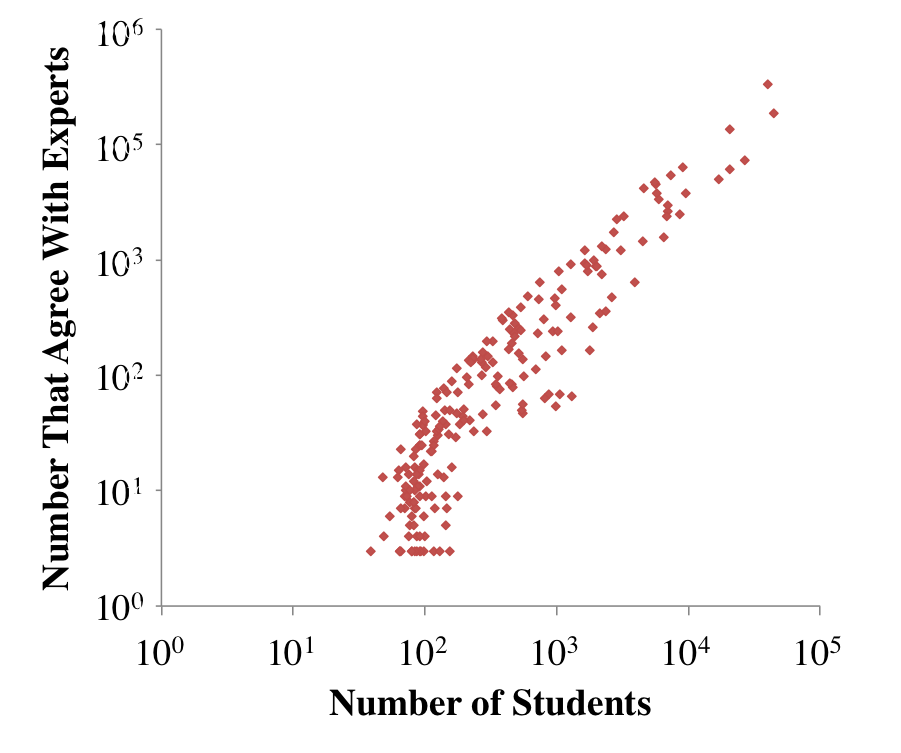
\includegraphics[width=0.5\columnwidth]{img/wrongVsPopularity.png}
\caption[Partial solution popularity vs probability of optimal progress]{How does node popularity relate to number of students who agree with experts?}
\label{fig:confidence}
\end{figure}


If we base our policy off of the transitions of students, we will often be trusting a group of learners that we know have already made a mistake. This biased sample limits our ability to understand the path-to-solution that \emph{would} have been the most popular \emph{if} partial solutions were all visited by ideal students. This raises a question: how can we know anything about a given partial solution that isn't collected solely from the students that submit said partial solution? 

One answer to that question is that we know the relative popularity of a partial solution based on how often it was submitted. Unlike transition counts, which sample from a biased population, the number of times a partial solution is seen in our dataset, ``partial solution counts," reflect a property of that partial solution for the average student in the dataset. A relatively high popularity suggests that the average student in the sample found the partial solution to be a useful way-point on a path-to-solution. A relatively low popularity suggests that the average student did not. By creating algorithms based off of this statistic we can avoid the confound that arises from the uneven distribution of ability across partial solutions.

Even if we make the assumption that partial solution counts reflect a global desirability of that partial solution how can we turn that intuition into a PSP? The solution is not as easy as: for any partial solution, chose the legal move such that the next partial solution has a high count. That strategy, more often than not, would encourage the student to delete any progress they have made. The most popular partial solution is the empty program and partial solutions which are further from the empty program tend to be less popular. Instead, to generate a PSP we must seek a balance between visiting desirable partial solution and making forward progress. We believe that teachers strike this balance by considering the entire path that they would expect a student to go down. Algorithmically this can be interpreted as searching for an optimally desirable path-to-solution. Once a path-to-solution is decided upon, the PSP function is simply the first step in that path.

We propose a desirable path theory which assumes that (a) desirability of a partial solution to the average student is a function of historical counts and (b) experts suggest that learners make progress along the most desirable path-to-solution. We present two algorithms that derive from this theory. 

\subsubsection{Poisson Path}

The first algorithm that we propose based on the desirable path theory is the Poisson Path.

We define the Poisson Path from a partial solution $s$ to be the path from $s$ to a perfect solution with the smallest expected time to be generated by the average successful student. We assume that the amount of time required for an average student to generate a partial solution is a Poisson process whose rate parameter can be estimated via the partial solution count from the student's population. This assumption is founded in the belief that the prototypical student prefers partial solutions that are easy to generate.

Given these assumptions the Poisson Path $\gamma(s)$ is:
\begin{align*}
\gamma(s)=\argmin_{p \in Z(s)}{\sum_{x \in p}{\frac{1}{\lambda_x}}}
\end{align*}
Where $Z(s)$ are all the paths-to-solution from $s$ and $\lambda_x$ is the number of times partial solution $x$ is seen in successful student data. To generate a PSP we set $\pi(s)$ to be the first partial solution in the path $\gamma(s)$. 



\begin{defo}
Poisson Path. \\ 
Let $G$ be a graph traversed by agents. Assume for a node $x \in G$, the time required for an agent to visit that node varies as an $exponential(\lambda_x)$ where $\lambda_x$ is a Poisson rate parameter. 

The expected time until an agent visits a given node $x$ is $\frac{1}{\lambda_x}$ and the expected time until an agent generates each node in a path $p$ is 
$\sum_{x \in p}{\frac{1}{\lambda_x}}$


The Poisson Path is the path from a node $s$ to a terminal with the smallest expected time required to be generated by an agent. Of all the paths $Z(s)$ from $s$ to the terminal, the path with the smallest expected time is 
\begin{align*}
\gamma(s)=\argmin_{p \in Z(s)}{\sum_{x \in p}{\frac{1}{\lambda_x}}}
\end{align*}
\label{pcpDef}
\end{defo}

Computing the Poisson Path can be solved using a simple reduction to Dijkstra's shortest path algorithm. We construct a graph where for all legal transitions $a \rightarrow b$ we add an edge with cost $\frac{1}{\lambda_b}$. A Dijkstra search for the shortest path to any solution over this graph will return the Poisson Path. Dijkstra's algorithm is easy to implement and runs in $O(n\log n)$ time for a graph with $n$ partial solutions. To prevent repeat submissions from having an undue influence on our partial solution counts we remove all cycles from student series before we count occurrences.


\subsubsection{Independent Probable Path}
A second algorithm that we propose based on the desirable path theory, is the Independent Probable Path. 

This algorithm tries to find the path-to-solution from a given partial solution that would have been the most probable for an average successful student who we would hypothetically start at that partial solution. For the average student we do not know partial solution transition probabilities. We instead know that the probability of the average student submitting a partial solution is proportional to the partial solution count. Using these submission probabilities we can calculate the markov-zero most likely path-to-solution for a randomly sampled student in the class. The Independent Probable Path $\gamma(s)$, is calculated as:
\begin{align*}
\gamma(s)&=\argmax_{p \in Z(s)}{\prod_{x \in p}{p(\psi_t = x)}} \\
         &=\argmax_{p \in Z(s)}{\sum_{x \in p}{\log(\frac{\lambda_x}{k})}}\\
         &=\argmin_{p \in Z(s)}{\sum_{x \in p}{-\log(\frac{\lambda_x}{k})}}
\end{align*} 


Where $Z(s)$ are all paths in the legal move graph from $s$ to the solution, $\lambda_x$ is the count of successful students who submitted $x$ and $k$ is the total number of submissions. This algorithm can also be reduced to an instance of Dijkstra's shortest path. 

\subsection{Baseline Algorithms}
Several algorithms for generating PSPs have been proposed in recent publications. Here we provide a brief overview of the algorithms and any modifications that were made to better fit the algorithms to the Code.org context. We also explore a series of simpler, direct measures. 

\subsubsection{Markov Decision Problem}
As proposed by Barnes and Stamper we can generate a PSP by formulating student transitions as a Markov Decision Problem (MDP) and learning an optimal policy. An MDP is defined by specifying states, actions, rewards over states and transition probabilities. In the Barnes et al formulation the states are the set of partial solutions, actions are the legal changes to a program allowed in the interface and the reward of a partial solution is set to be 100 if it is a correct answer, 0 otherwise. Of note, the transition probability between partial solutions $a$ and $b$ is defined as $p(\psi_{t+1} = b | \psi_t = a)$.

In a standard MDP the transition probability is the chance of ending up in a state given one's previous state \emph{and} an action the policy decided to perform. Applied to this setting we would need to know the probability of a student going from one partial solution to another \emph{if} we were to suggest a particular next state. In the historical data available to Barnes et al and in the Code.org context that conditional probability is unknown; we can't observe how our suggestions would effect student transitions. Instead, as in Barnes et al, we assume that a student's transition probability is independent of the partial solution we chose for them. The MDP has a single hyper-parameter, the discount factor. We use standard value iteration \cite{shapley1953stochastic} inference on the MDP which results in a PSP. 

\subsubsection{Rivers Policy}
In a paper recently published Rivers et al provided an algorithm for choosing the ideal next step \cite{rivers2014automating}. For a given partial solution, the algorithm computes a score for all potential next partial solutions and selects the argmax. The score is a weighted sum of features. We adapted their score to utilize the legal move graph which results in the following policy function:
\begin{align*}
\pi(x) = \argmax_{n \in N(x)} {\theta_0 \lambda_n + \theta_1 (1 - \delta(n, g)) + \theta_2 v(n)}
\end{align*}
Where $N(x)$ are the neighbors of $x$ in the legal move graph, $\lambda_n$ is the popularity of the partial solution, $\delta(n, g)$ is the minimum Abstract Syntax Tree edit distance between a neighbor $n$ and a correct answer $g$ and $v(n)$ is the unit-test score of the neighbor. Though specific settings for parameters $\theta$ are provided in the paper, after trying the values given we considered the weights to be hyper-parameters. 



\subsubsection{Static Analysis}
Given the simple nature of the hour of code problems, especially \Pa, we hypothesized that the optimal PSP could be chosen by a static analysis solution. For \Pa there was a single optimal sequence of commands that solved the maze. Given any partial solution, we believed that the expert labels could be perfectly predicted by a sequence alignment algorithm which compares the sequences of actions in the partial solution to the answer and selects the first divergence. We did our best to statically recreate human labels for \Pa. The algorithm allowed for reductions of equivalent blocks of code and had different insert and delete costs depending on relative position in the sequence. This algorithm was originally developed to generate gold standard data.


\subsubsection{Most Likely Next}
For each partial solution $x$, select the partial solution that most successful students transitioned to from $x$. This is equivalent to choosing the next state that has maximal probability $\pi{(x)} = \argmax_{n}{p(\psi_{t+1} = n | \psi_t = x)}$. 

\subsubsection{Most Common Path}
Find the the most common entire path to a solution in the dataset and set $\pi(x)$ to be the first partial solution in the path from $x$ to the correct answer.

\subsubsection{Expected Success}
For each partial solution $x$, select the legal next partial solution $y$ that maximizes the probability of a student arriving at the final answer given that they transition from $x$ to $y$. 

\subsubsection{Min Time}
Since all of our data was timestamped, for a given partial solution $x$ we can compute the expected time $J(x)$ between when a student submits $x$ and when they submit the correct solution. We chose $\pi(x) = \argmin_{n \in N(x)}J(n)$ to be the legal next partial solution that has minimal expected time until the student arrives at the solution.

\subsubsection{Ability Model}

We modified the inference algorithm for an item response model with unknown correct answers presented by Whitehill et al to learn a problem solving policy \cite{whitehill2009whose}. Let $t_j$ be the true next step for partial solution $j$. Let $\alpha_i$ be the ability of student $i$ and let $\beta_j$ be the difficulty of choosing right answer for partial solution $j$. Let $l_{ij}$ be the next step taken by student $i$ from state $j$. We model the probability of student $i$ being correct on item $j$ to be:
\begin{align*}
p(l_{ij} = t_j | \alpha_i, \beta_j) = \frac{1}{1 + e^{\alpha_i \beta_j}}
\end{align*}

We chose values for $\alpha$, $\beta$ and $t$ that best fit the data using expectation maximization. The policy was set as $\pi(x) = t_x$.





\subsection{Evaluation}
All ten of the algorithms listed--the Desirable Path algorithms, the previously proposed algorithms and the vanilla baseline algorithms--were run and the PSPs that they generated were tested against the gold standard data that we had collected.

For both \Pa and \Pb we use the gold standard data collected to generate an expert map $t : T \rightarrow S$ where $T \subset S$ is the set of partial solutions annotated by experts. For each partial solution $k \in T$, $t(k)$ is the set of partial solutions that experts say a student should ideally transition to from $k$.

To evaluate a PSP $\pi$ we calculate the percent of overlap between the policy and the expert map, weighted by number of students who submitted partial solutions. Let $\lambda_k$ be the number of students that submitted partial solution $k$. We computed accuracy as:
\begin{align*}
acc_\pi &= \frac{\sum_{k \in T}{\lambda_k \delta(k)}}{\sum_{k \in T}{\lambda_k}}\\
\delta(k) &= 
\begin{cases}
    1,  & \text{if } \pi(k) \in t(k)\\
    0,  & \text{otherwise}
\end{cases}
\end{align*}


Four of the baseline policies that we tested (MDP, Static Analysis, Rivers Policy and Ability Model) had hyper-parameters. To maximally benefit the baseline methods we optimize hyper-parameters with respect to accuracy on \Pa. This means that for those algorithms, it is possible that their performance numbers will be artificially higher on \Pa due to over-fitting.

\section{Results}

The best algorithm for both \Pa and \Pb was the Poisson Path policy which had accuracy of 95.9\% and 84.6\% respectively despite making the desirable path assumptions and only using submission counts. Indeed, the second best performing algorithm also made such assumptions and had almost identical accuracies. See table \ref{tab:results1} for the full results. The structure of the policies learned by the Desirable Path Algorithms tended to push students towards a backbone pathway of partial solutions. This pattern is visible in figure \ref{fig:policy} which depicts the Poisson Path PSP for \Pa\hspace{-0.5mm}. You can see the backbone through partial solutions [10, 9, 1, 2, 0] that the algorithm favored. 

\begin{table}[t]
  \centering
  \ra{1.3}
\begin{tabular}{@{}lll}
     \toprule
        & \tabhead{\Pa Accuracy} & \tabhead{\Pb Accuracy}  \\
    \midrule
    \tabhead{Algorithm} \\
    \hspace{1mm} 
    Random & 8.2\% & 4.3\% \\
    \hspace{1mm} 
    Shortest Path & 49.5\% & 33.6\% \\
    \hspace{1mm}
Min Time & 67.2\%  &  42.2\%\\
    \hspace{1mm}
    Rivers Policy$^\dagger$ & 72.9\% & 78.2\% \\ 
    \hspace{1mm}
    Expected Success & 77.9\% & 56.2\% \\
    \hspace{1mm}
    MDP$^\dagger$ & 80.5\% & 47.6\%\\
    \hspace{1mm}
    Most Common Next & 81.1\% & 49.0\% \\
    \hspace{1mm}
    Static Analysis$^\dagger$ & 86.3\% & - \\
    \hspace{1mm}
    Most Popular Path & 88.3\% & 52.8\% \\
    \hspace{1mm}
    Ability Model & 88.4\% & 63.3\% \\
    
    \hspace{1mm}
     Independent Probable Path $^\ddagger$ & \textbf{95.5}\% & \textbf{83.3}\% \\
    \hspace{1mm}
    Poisson Path $^\ddagger$ & \textbf{95.9}\% & \textbf{84.6}\% \\
    \tabhead{Variation} \\
    \hspace{1mm}
     Unconditioned on Success & 72.2\% & 68.3\% \\
    \hspace{1mm}
     No Interpolation & 86.8\% & 70.5\% \\
    \hspace{1mm}
     Allow Cycles & 94.3\% & 82.0\% \\
    \hspace{1mm}
     Poisson Interpolation & 94.6 \% & 83.2\% \\
    \bottomrule
  \end{tabular}
  \captionof{table}[Problem solving policy accuracies]{Percent submissions with the ground truth edge correctly predicted. $^\dagger$ Algorithms applied to learning PSP's in other papers. $^\ddagger$ Desirable Path Algorithms.}
  \label{tab:results1}
  \end{table}

The other algorithms had notably lower scores. Interestingly, algorithms that were based on transition dynamics, eg MDP and Most Common Next were less effective even though we  had enough historical data to accurately approximate transition probabilities. This result seemed related to the observation that outside the mainstream paths-to-solution students systematically made transitions which disagreed with expert suggestions. We observed that for most partial solutions, the majority of students did not take an action which agreed with the expert label. In fact for \Pa\hspace{-0.5mm}, for over 51\% of the expert labelled partial solutions, the most popular next partial solution was not one that experts said students should transition to, and for 34\% of labelled partial solutions, the incorrect most popular next step was over three times as popular as any expert recommended next step. 


\begin{figure}
\centering
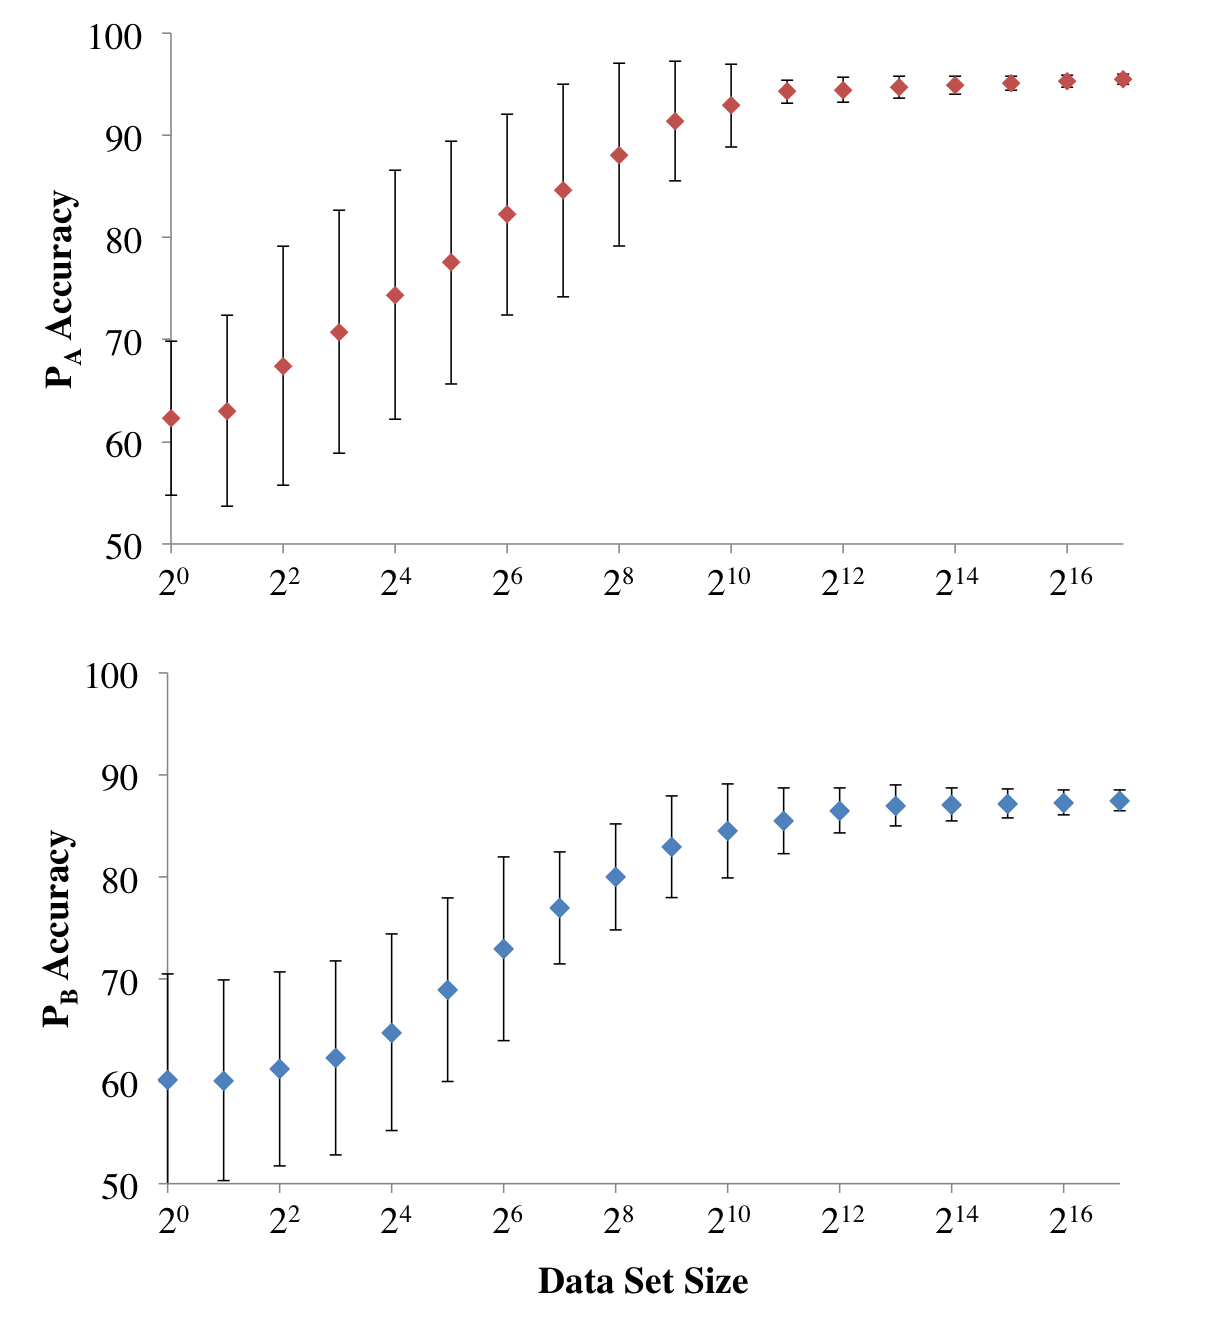
\includegraphics[width=0.5\columnwidth]{img/lcs}
\caption[Poison path learning curve]{Learning curve for \Pa (above) and \Pb (bellow). Students are subsampled randomly from dataset. Error bars are standard error.}
\label{fig:learningCurve}
\end{figure}


While the Rivers Policy performed well on the \Pb in many instances in \Pa it would suggest a student undo something constructive from their partial solution. The optimal static analysis algorithm was worse than the best trajectory based algorithm and it would have been very difficult to design such a system for \Pb\hspace{-0.5mm}. There is a lot of nuance that goes into deciding what a student should do. The experts seem to be working in a formulaic way, but it is very difficult to codify their decision making. 

There are several variations of the Poisson Path that we tested to understand what preprocessing was most important. The two steps that were necessary were: (1) interpolate each student series over the graph of single legal moves and (2) condition node counts on success (see table \ref{tab:results1}). Removing cycles from student partial solution series is less important. We applied the same pre-processing for all algorithms tested.

We ran an experiment to understand the effect of dataset size on accuracy. On both \Pa and \Pb we subsampled students from our dataset and reran the entire policy learning process (including the interpolation). The policy generated by the subsampled students was evaluated for accuracy on the same gold standard expert data. We started with a training dataset size of two students and continually doubled the number of students. For each size we repeated the experiment 100 times to estimate accuracy mean and standard deviation.  See figure \ref{fig:learningCurve}. Even if we were given historical data from substantially fewer students the Poisson Path PSP would have had comparable accuracy. With a dataset of only two thousand students accuracy is similar to the results from running the algorithm on hundreds of thousands of students. While two thousand students may be sufficient, as more data is collected the algorithm monotonically improves in accuracy and accuracy variance. Since the Poison Path algorithm can be cast as an instance of Dijkstra's shortest path the running time will be reasonable even for courses that are orders of magnitude larger than the Hour of Code.



\subsection{Summative Assessment}

\begin{figure*}[!ht]
\begin{center}
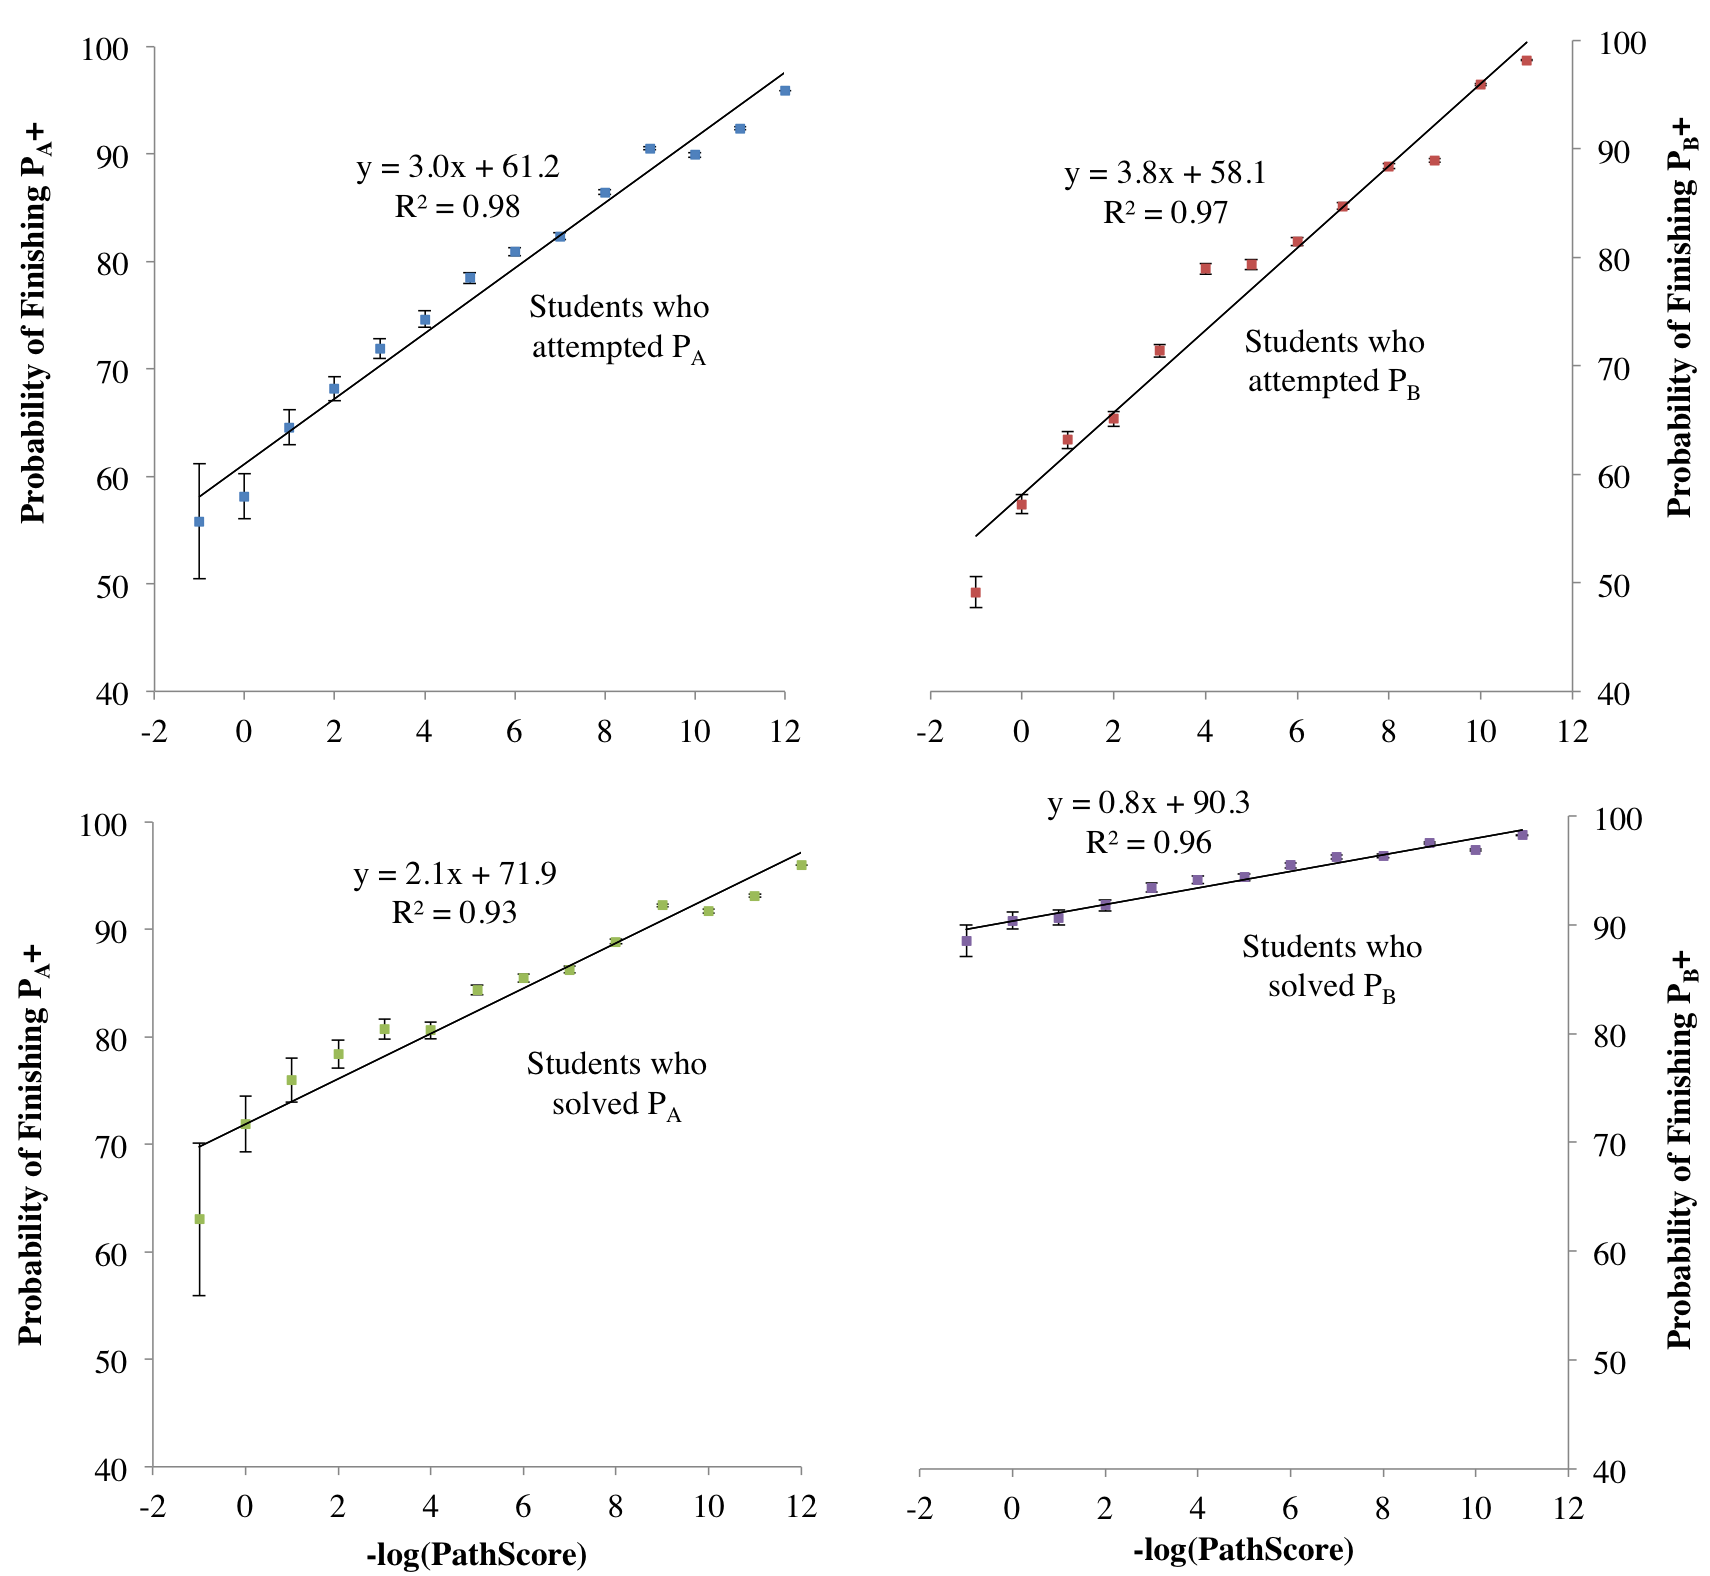
\includegraphics[width=1.0\textwidth]{img/future}

\end{center}
\caption[Poisson path score predicts completion]{Student path scores vs probability of completion of subsequent problems. Error bars are standard error.
 }
\label{fig:predacc}
\end{figure*}

The same insights that allow us to predict how experts would suggest students make forward progress can be used to understand how well each student progressed through the assignment. The desirable path theory that inspired both the Poisson Path and the Independent Probable Path algorithms suggests a statistic that can be measured per student. Assuming that path counts of a partial solution are a function of desirability, we can then calculate the desirability of the path of partial solutions a student took through as they worked through a challenge. 

Based on the Poisson interpretation of desirability used in the Poisson Path, we define the ``path score" of a student's series $T$ to be the time we expect an average successful student would take to complete the series. Assuming that each state is generated via a Poisson process, expected time until we see the series of states that constitute a path is the sum of the inverse of the rate of each partial solution:
\begin{align*}
 pathScore(T) = \sum_{x \in T}{\frac{1}{\lambda_x}}
\end{align*}
 We calculated the path score for each student and explored how the scores were related to the probability that the student would complete the next challenge. For example \Pa is the fourth challenge in the Hour of Code. We computed a path score for each student that completed \Pa and observed which of those students went on to solve the fifth challenge (\Pa+).



From simple visualization it was clear that the negative log of the path score had a strong linear relationship with probability of completing the next challenge for students in both \Pa and \Pb\hspace{-0.5mm}. For the population of students who attempted \Pa, their probability of completing the next challenge \Pa\hspace{-0.5mm}+ increased by 3\% with each per unit increase in $-\log(pathScore)$. Linear regression between $\log(pathScore)$ and the probability of completing the next challenge had an $R^2$ of 0.98. Learners with the worst paths had a 58\% chance of completing the next problem and learners with the best paths had a 95\% chance: an effect size of 37pp. \Pb similarly had an straight line pattern ($R^2$ = 0.97) and an effect size of 43pp. See figure \ref{fig:predacc}.

This trend is especially interesting when we only look at the scores of students who arrived at a solution to the challenge from which we calculate the path scores. These are the students who, if it were a traditional classroom, would have received a perfect grade. For \Pa the successful students with the worst and the best path scores had a 25.1pp difference in the probability of completing the subsequent problem. Again there was a linear relationship between the negative log of the path score and probability of success ($R^2$ = 0.93). \Pb also had a linear relationship ($R^2$ = 0.96), with an effect size that was 9.7pp between the best and the worst path scores. It seems plausible that many students who may have disengaged from the curriculum because of a factor related to low path score may not have stayed in the course until the 18th challenge. In both problems the Path Score shows predictive signal towards retention beyond what we could know from simply observing whether a students solved the challenge.

\subsection{Generating Hints}

In the introduction of this paper we proposed that the challenge of autonomously providing hints could be decoupled into (1) Deciding how a learner should make forward progress and (2) Choosing how to communicate that information to the student such that they improve on a learning objective. Given that we can solve the first task sufficiently well, we are  pursuing research on the second: how to turn our PSP into hints. This latter task combines education and UI decisions.

Having a PSP for a given challenge substantially simplifies the task of generating hints. It tells the hint generation algorithm which part of a student's current partial solution they should work on, and how they should modify their work. Often, students have multiple issues. A policy allows an automated system to know what is the first issue the student should work on. Moreover, knowing the exact edit we believe an expert would like a student to make means that generating a hint is reduced to deciding how directly we should tell the student what to do. Based off of a simple template we turned $\pi(x)$ into English text hints. We are currently running an A/B study with thousands of students where they either receive hints generated autonomously from the policy, hints hand-crafted by humans, or placebo hints. 

\section{Discussion}

One of the more surprising results of this research is that even with hundreds of thousands of students, it turns out that many reasonable statistics on learner trajectories are not particularly useful for predicting what experts say is the correct way forward. Most interestingly, the transitions that learners take after encountering a problem do not tend to correspond with what experts think learners should do. The wisdom of the crowd of learners, as seen from this angle, is not especially wise. This result raises the question: What is so good about the Poisson Path? Why does it, and the Independent Probable Path work when other methods do not? In designing both of the Desirable Path Algorithms, we followed our intuition that a useful algorithm would be able to predict what an \emph{average} successful student would do if we were to place her in a partial solution. We first assumed that partial solution submission counts are uniquely important as they are a statistic which reflects how desirable a partial solution is to the \emph{average} student (or rather the inverse is a measure of how relatively undesirable). Many baseline algorithms instead relied on transition counts, but that number captures what the biased population of students who had arrived at a given partial solution, \emph{not} the average student, would do. Previous research suggests that transition-based algorithms are limited by lack of data. We now believe that their shortcomings are instead a result of reliance on subpopulations with systematic predispositions. When designing the Desirable Path Algorithms we also assumed that when deciding on a next step it is best to search for an entire path to solution. Many baseline algorithms only consider neighboring partial solutions and do not see the bigger picture. We propose that the success of the Desirable Path Algorithms is evidence that both assumptions are important, operable properties of historical student trajectories. 

Code.org is a compelling case study as tens of millions of students are expected to use the website next year. However, it is only one course and as such is not a proof of our ability to provide feedback for general richly-structured assignments. Even for the Hour of Code where the problems are simple and there are huge numbers of students, the solution space is almost too disperse for statistical methods. Though there may be millions of students, outside the most common partial solutions there is a sharp drop-off in both the density of students per partial solution, and the proportion of students who took reasonable next steps.  For more complicated programming tasks, or written language tasks, there would be too few students that would submit the same partial solutions \cite{huang2013syntactic}; feedback based on historical patterns over raw partial solutions has its limits. One way in which we could further extend the boundary of assignments for which we could provide at scale feedback using the Desirable Path Algorithms would be to develop a better representation for partial solutions and/or a more intelligent way to find patterns in submissions. In general the AI challenges in education are hard and the field can make faster progress if we decouple the evaluation of machine learning tasks so that we can make progress without continuously paying the heavy cost of user studies.

A limitation of our approach is that it is not clear that students need hints and it is not clear that pushing a student towards the answer is the right objective \cite{roll2014benefits}. A lot of learning happens when we struggle and go off on tangents. In the Code.org context, hints that push students towards the solution are useful because the goal of the Hour of Code is primarily motivation. The course intends to provide learners with an exposure to programming. Being able to give a stuck student a hint is useful for fostering retention and interest in the subject. One way to approach the uncertainty of knowing whether a hint would be useful for a student is through a reinforcement-agent hint-giving system. Such a system would be integrated into the website and would dynamically decide whether to give a hint (and if so, which hint). There are well studied ways to balance the need to explore the impacts of giving different hints to learners at different times, and to exploit what is known to work. 

Beyond the capacity to generate hints, the process of finding signals in historical data has interesting side-products. The most important corollary we presented is that the same intuition that guides generating PSPs can help us understand individual learners and predict retention. Piech et al found prototypical clusters of ways in which students solve problems that were predictive of exam scores \cite{piech2012modeling}. This paper goes beyond that result by calculating a continuous valued path score which can make more fine grained predictions. Our ability to predict both retention and teacher suggestions are results that lend credibility to one another. The Path Score metric has obvious utility as a diagnostic measure that could help identify learners that may need more attention. Of course, knowing that a student has a bad path score does not imply \emph{why} the student has a low probability of completing a subsequent challenge. It is only a correlation. It is not clean why Path Scores and probability of retention are exponentially related. One interpretation is that there is a monotonic ability scale and that each unit decrease in ability has compounding, and therefore exponential, impact on how well a student navigates through partial solutions. 

As interesting idea to try would be to using a recurrent neural network with one hot encoding of the unique partial solution over time.

There are more undiscovered patterns in how students navigate richly-structured assessments. Student trajectories remain a great mystery.

\subsection{Conclusion}

In this paper we explored ways to solve the machine learning question: how can we predict the way a teacher would encourage a student to make forward progress? The ability to make such prediction is useful for generating feedback at scale. We show that in the Code.org case study two algorithms with the same theoretical backing are accurate at recreating expert opinion. These algorithms can be applied to logs of learners working on problems for which there are no expert labels, and will produce an intelligent strategy for what learners ought to do. We then claim that the same theory can be used to calculate a statistic on how well a student navigated the assignment and show that this statistic predicts future retention. The way in which students solve problems is fertile ground for research in learning at scale. Instead of looking solely at a student's final answer, education of the future will take note of the journey the learner took to get there.